%%%%%%%%%%%%%%%%%%%%%%%%%%%%%%%%%%%%%%%%%
% Beamer Presentation
% LaTeX Template
% Version 1.0 (10/11/12)
%
% This template has been downloaded from:
% http://www.LaTeXTemplates.com
%
% License:
% CC BY-NC-SA 3.0 (http://creativecommons.org/licenses/by-nc-sa/3.0/)
%
%%%%%%%%%%%%%%%%%%%%%%%%%%%%%%%%%%%%%%%%%

%----------------------------------------------------------------------------------------
%	PACKAGES AND THEMES
%----------------------------------------------------------------------------------------

%\documentclass{beamer}
\documentclass[12pt, aspectratio=169]{beamer}
\usepackage{keynote-gradient}

\mode<presentation> {

% The Beamer class comes with a number of default slide themes
% which change the colors and layouts of slides. Below this is a list
% of all the themes, uncomment each in turn to see what they look like.

%\usetheme{default}
%\usetheme{AnnArbor}
%\usetheme{Antibes}
%\usetheme{Bergen}
%\usetheme{Berkeley}
%\usetheme{Berlin}
%\usetheme{Boadilla}
%\usetheme{CambridgeUS}
%\usetheme{Copenhagen}
%\usetheme{Darmstadt}
%\usetheme{Dresden}
%\usetheme{Frankfurt}
%\usetheme{Goettingen}
%\usetheme{Hannover}
%\usetheme{Ilmenau}
%\usetheme{JuanLesPins}
%\usetheme{Luebeck}
%\usetheme{Madrid}
%\usetheme{Malmoe}
%\usetheme{Marburg}
%\usetheme{Montpellier}
%\usetheme{PaloAlto}
%\usetheme{Pittsburgh}
%\usetheme{Rochester}
%\usetheme{Singapore}
%\usetheme{Szeged}
%\usetheme{Warsaw}

% As well as themes, the Beamer class has a number of color themes
% for any slide theme. Uncomment each of these in turn to see how it
% changes the colors of your current slide theme.

%\usecolortheme{albatross}
%\usecolortheme{beaver}
%\usecolortheme{beetle}
%\usecolortheme{crane}
%\usecolortheme{dolphin}
%\usecolortheme{dove}
%\usecolortheme{fly}
%\usecolortheme{lily}
%\usecolortheme{orchid}
%\usecolortheme{rose}
%\usecolortheme{seagull}
%\usecolortheme{seahorse}
%\usecolortheme{whale}
%\usecolortheme{wolverine}

%\setbeamertemplate{footline} % To remove the footer line in all slides uncomment this line
\setbeamertemplate{footline}[page number] % To replace the footer line in all slides with a simple slide count uncomment this line

\setbeamertemplate{navigation symbols}{} % To remove the navigation symbols from the bottom of all slides uncomment this line
}

\usepackage{graphicx} % Allows including images
\usepackage{booktabs} % Allows the use of \toprule, \midrule and \bottomrule in tables

%--------------------------------------------------------------------------------
%	TITLE PAGE
%--------------------------------------------------------------------------------

\title[Memristive brain]{Memristive brain} % The short title appears at the bottom of every slide, the full title is only on the title page

\author[Max Talanov, Evgeniy Zykov]{
  
\includegraphics[height=3cm]{ITIS_logo_bright}\\
  Max Talanov, Evgeniy Zykov
} 
\institute[ITIS: KFU] % Your institution as it will appear on the bottom of every slide, may be shorthand to save space
{
Machine cognition lab, Intellectual robotics department, ITIS \\ % Your institution for the title page
\medskip
\textit{max.talanov@gmail.com, evgeniy.zykov@kpfu.ru} % Your email address
}
\date{\today} % Date, can be changed to a custom date

\begin{document}

\begin{frame}
\titlepage % Print the title page as the first slide
\end{frame}

%-------------------------------------------------------------------------------
%	PRESENTATION SLIDES
%-------------------------------------------------------------------------------

%------------------------------------------------
\section{Knowledge map}
%------------------------------------------------

\begin{frame}
\frametitle{Knowledge map}
\begin{figure}
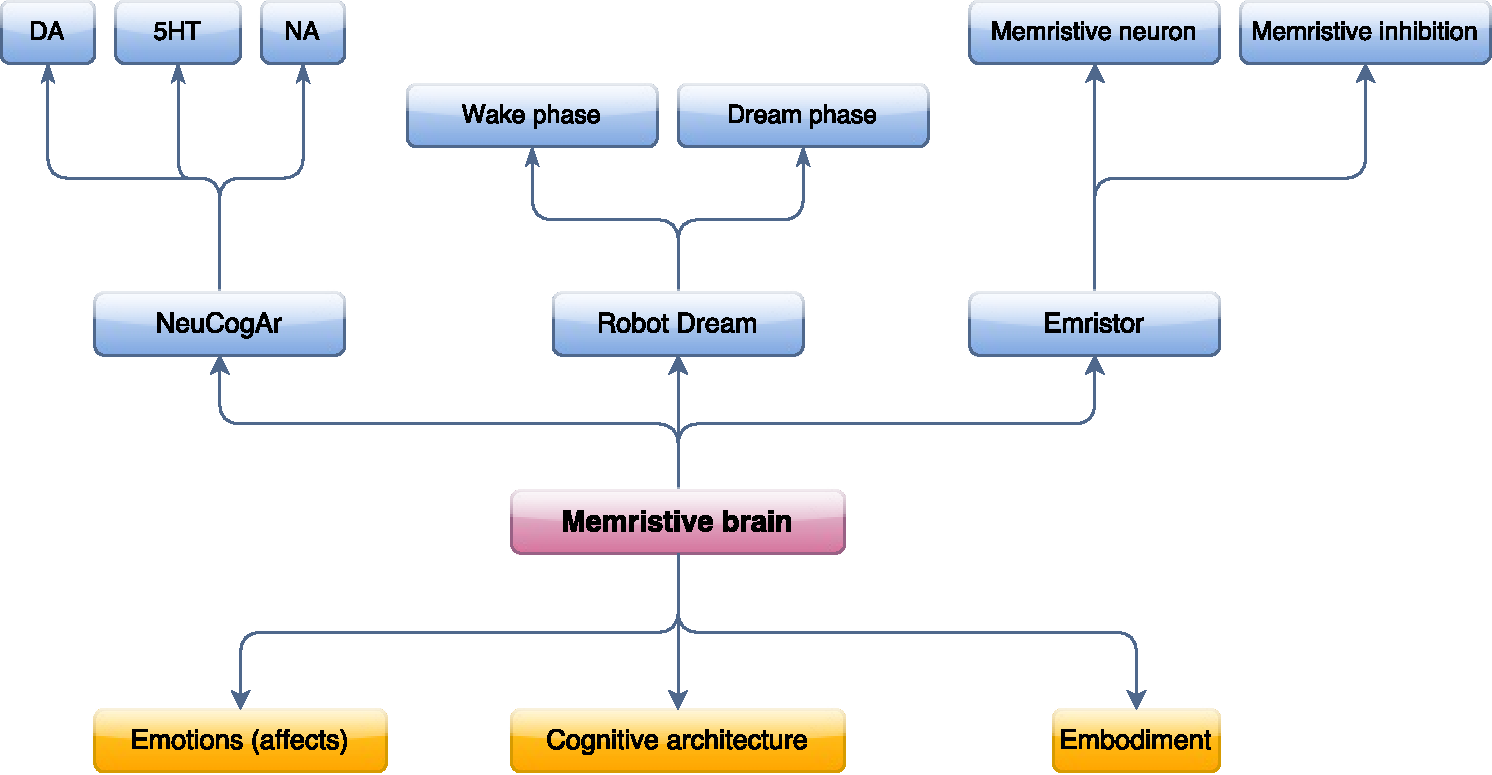
\includegraphics[width=0.7\linewidth]{knowledge_map}
\end{figure}
\end{frame}

%------------------------------------------------
\section{AGI approach}
%------------------------------------------------

\begin{frame}
\frametitle{Metafor}
\begin{columns}[c] % The "c" option specifies centered vertical alignment while the "t" option is used for top vertical alignment
\column{.5\textwidth} % Left column and width
\begin{figure}
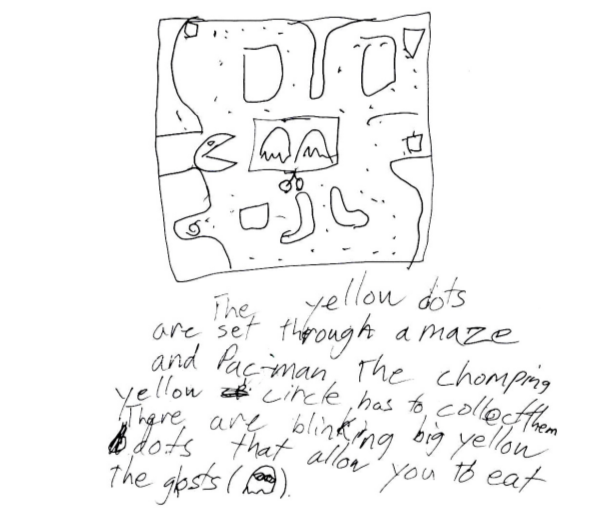
\includegraphics[width=1.0\linewidth]{metafor}
\end{figure}
\column{.5\textwidth}
\begin{figure}
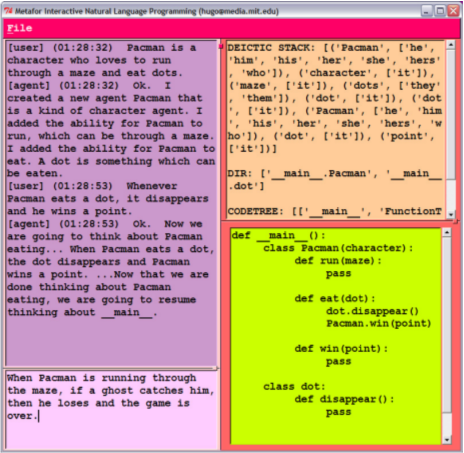
\includegraphics[width=1.0\linewidth]{metafor_gui}
\end{figure}
\end{columns}
\end{frame}

%------------------------------------------------
%------------------------------------------------

\begin{frame}
  \frametitle{Metafor video}
  \ldots
\end{frame}

%------------------------------------------------
%------------------------------------------------

\begin{frame}
  \frametitle{AGI problems}
  \begin{itemize}
    \item System is too fragile.
    \item Not capable of the adaptation to the real life.
    \item Not capable of thinking ...
    \item Too many stupid rules.
  \end{itemize}
\end{frame}

%------------------------------------------------
\section{Emotions}
%------------------------------------------------

\begin{frame}
\frametitle{Consciousness $\Rightarrow$ Emotions}
\begin{columns}[c] % The "c" option specifies centered vertical alignment while the "t" option is used for top vertical alignment

\column{.45\textwidth} % Left column and width
\textbf{Human:}
\begin{itemize}
\item Cognition $\Rightarrow$ Consciousness $\Rightarrow$ Emotions
\end{itemize}

\textbf{Machine:}
\begin{itemize}
\item Cognition $\Rightarrow$ Consciousness $\Rightarrow$ Emotions
\end{itemize}

\column{.6\textwidth} % Right column and width
%------------------------------------------------
\begin{figure}
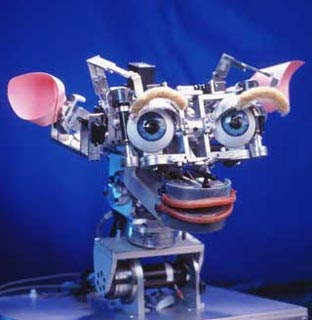
\includegraphics[width=0.8\linewidth]{Kismet_312}
\end{figure}
%------------------------------------------------
\end{columns}
\end{frame}

%------------------------------------------------
%------------------------------------------------

\begin{frame}
\frametitle{Mammalian emotions}
\begin{figure}
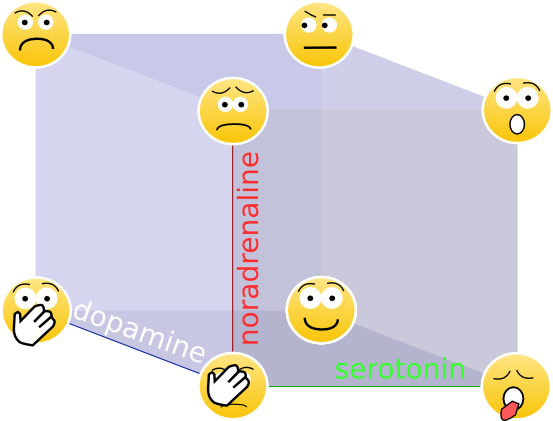
\includegraphics[width=0.7\linewidth]{cube_of_emotional_parameters}
\end{figure}
\end{frame}

%------------------------------------------------
%------------------------------------------------

\begin{frame}
\frametitle{NeuCogAr: robot emotions}
\begin{figure}
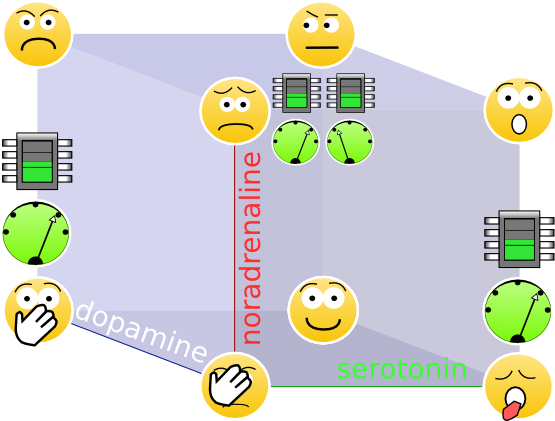
\includegraphics[width=0.7\linewidth]{cube_of_emotional_parameters_machine}
\end{figure}
\end{frame}

%------------------------------------------------
%------------------------------------------------

\begin{frame}
  \frametitle{Emotions $\Rightarrow$ computational processes}

\emph{Computing power utilization} overall load of the computational system is influenced by dopamine and serotonin that makes cortex fire spikes more actively.\\
\emph{Computing power distribution}(computing processes distribution or load balancing) is influenced by noradrenaline the higher is noradrenaline more computing processes should be concentrated on current activity.\\
\emph{Working memory}(short term) distribution is influenced by noradrenaline as neurotransmitter regulating attention.\\
\emph{Learning} is impacted by serotonin and dopamine: dopamine plays major role in activation of previously remembered patterns and serotonin in pattern generation.\\
\end{frame}

%------------------------------------------------
%------------------------------------------------

\begin{frame}
\frametitle{Simulation of emotions}
\begin{figure}
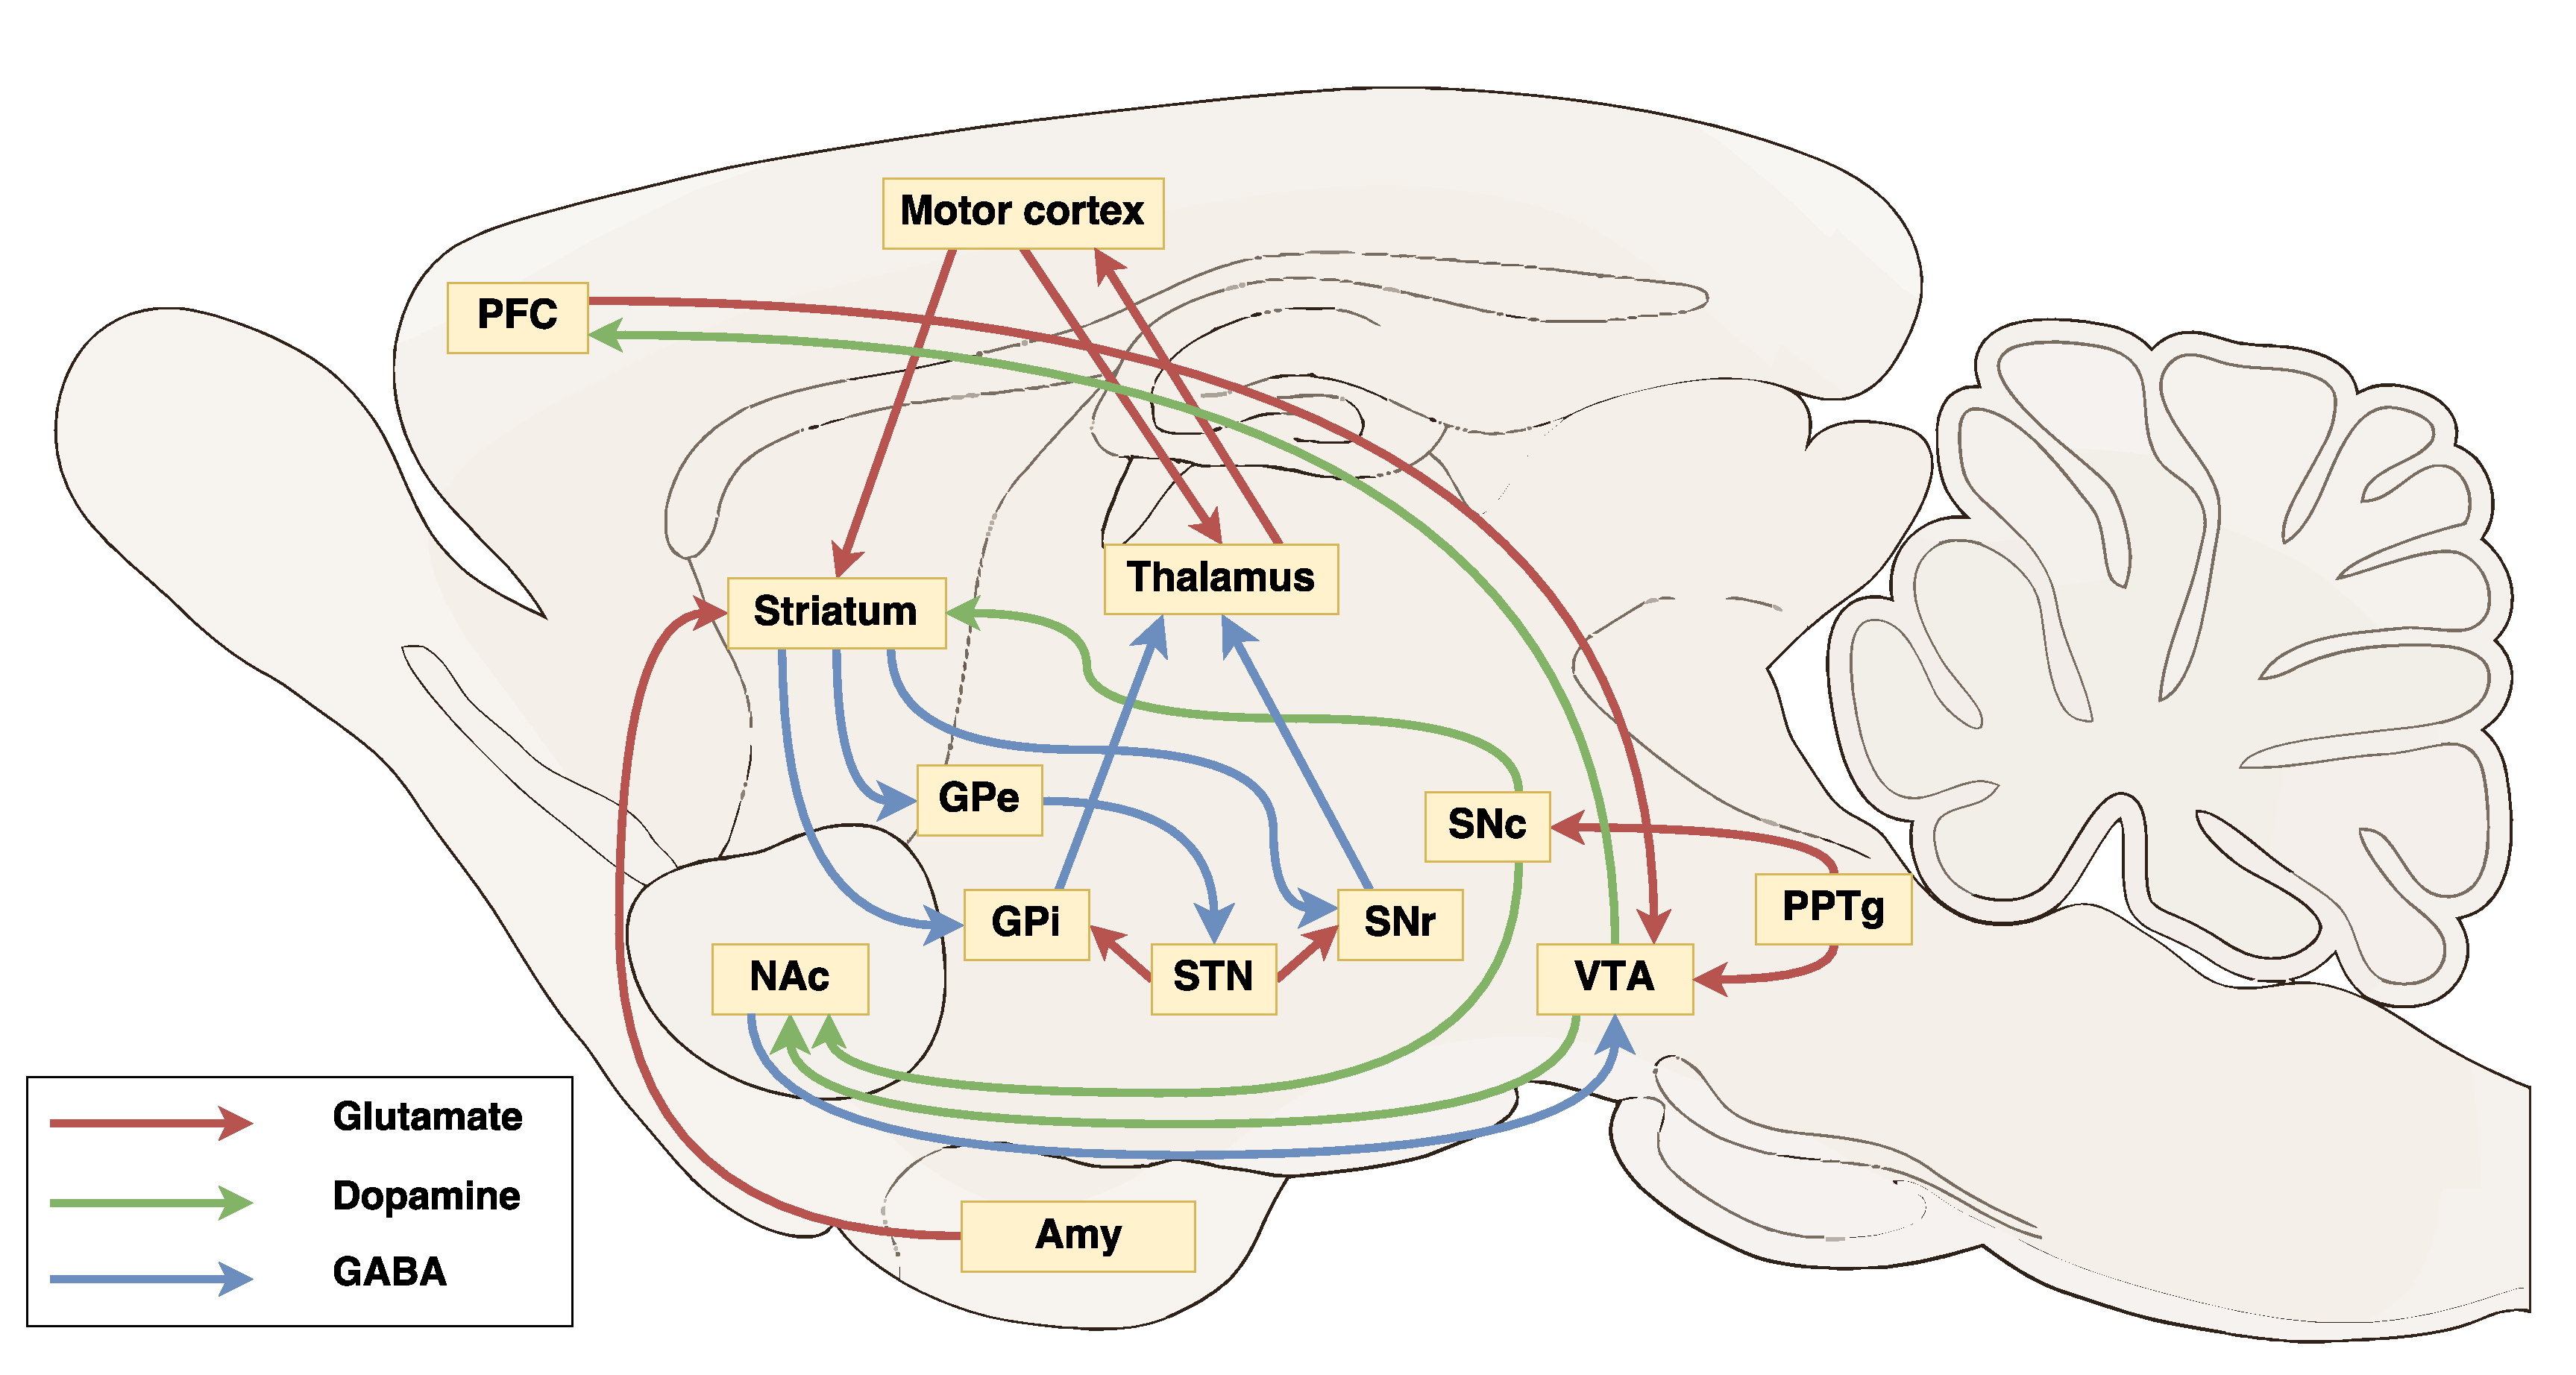
\includegraphics[width=0.99\linewidth]{rat_da}
\end{figure}
\end{frame}

%------------------------------------------------
%------------------------------------------------

\begin{frame}
\frametitle{Nigrostriatal pathway}
\begin{figure}
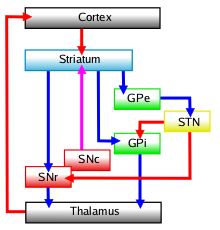
\includegraphics[width=0.45\linewidth]{nigrostriatal}
\end{figure}
\end{frame}

%------------------------------------------------
%------------------------------------------------

\begin{frame}
\frametitle{Dopamine pathways diagram}
\begin{figure}
\includegraphics[width=0.8\linewidth]{dopamine_diagram}
\end{figure}
\end{frame}

%------------------------------------------------
%------------------------------------------------

\begin{frame}
\frametitle{Serotonin pathways diagram}
\begin{figure}
\includegraphics[width=0.88\linewidth]{serotonin_diagram}
\end{figure}
\end{frame}

%------------------------------------------------
%------------------------------------------------

\begin{frame}
\frametitle{Noradrenaline pathways diagram}
\begin{figure}
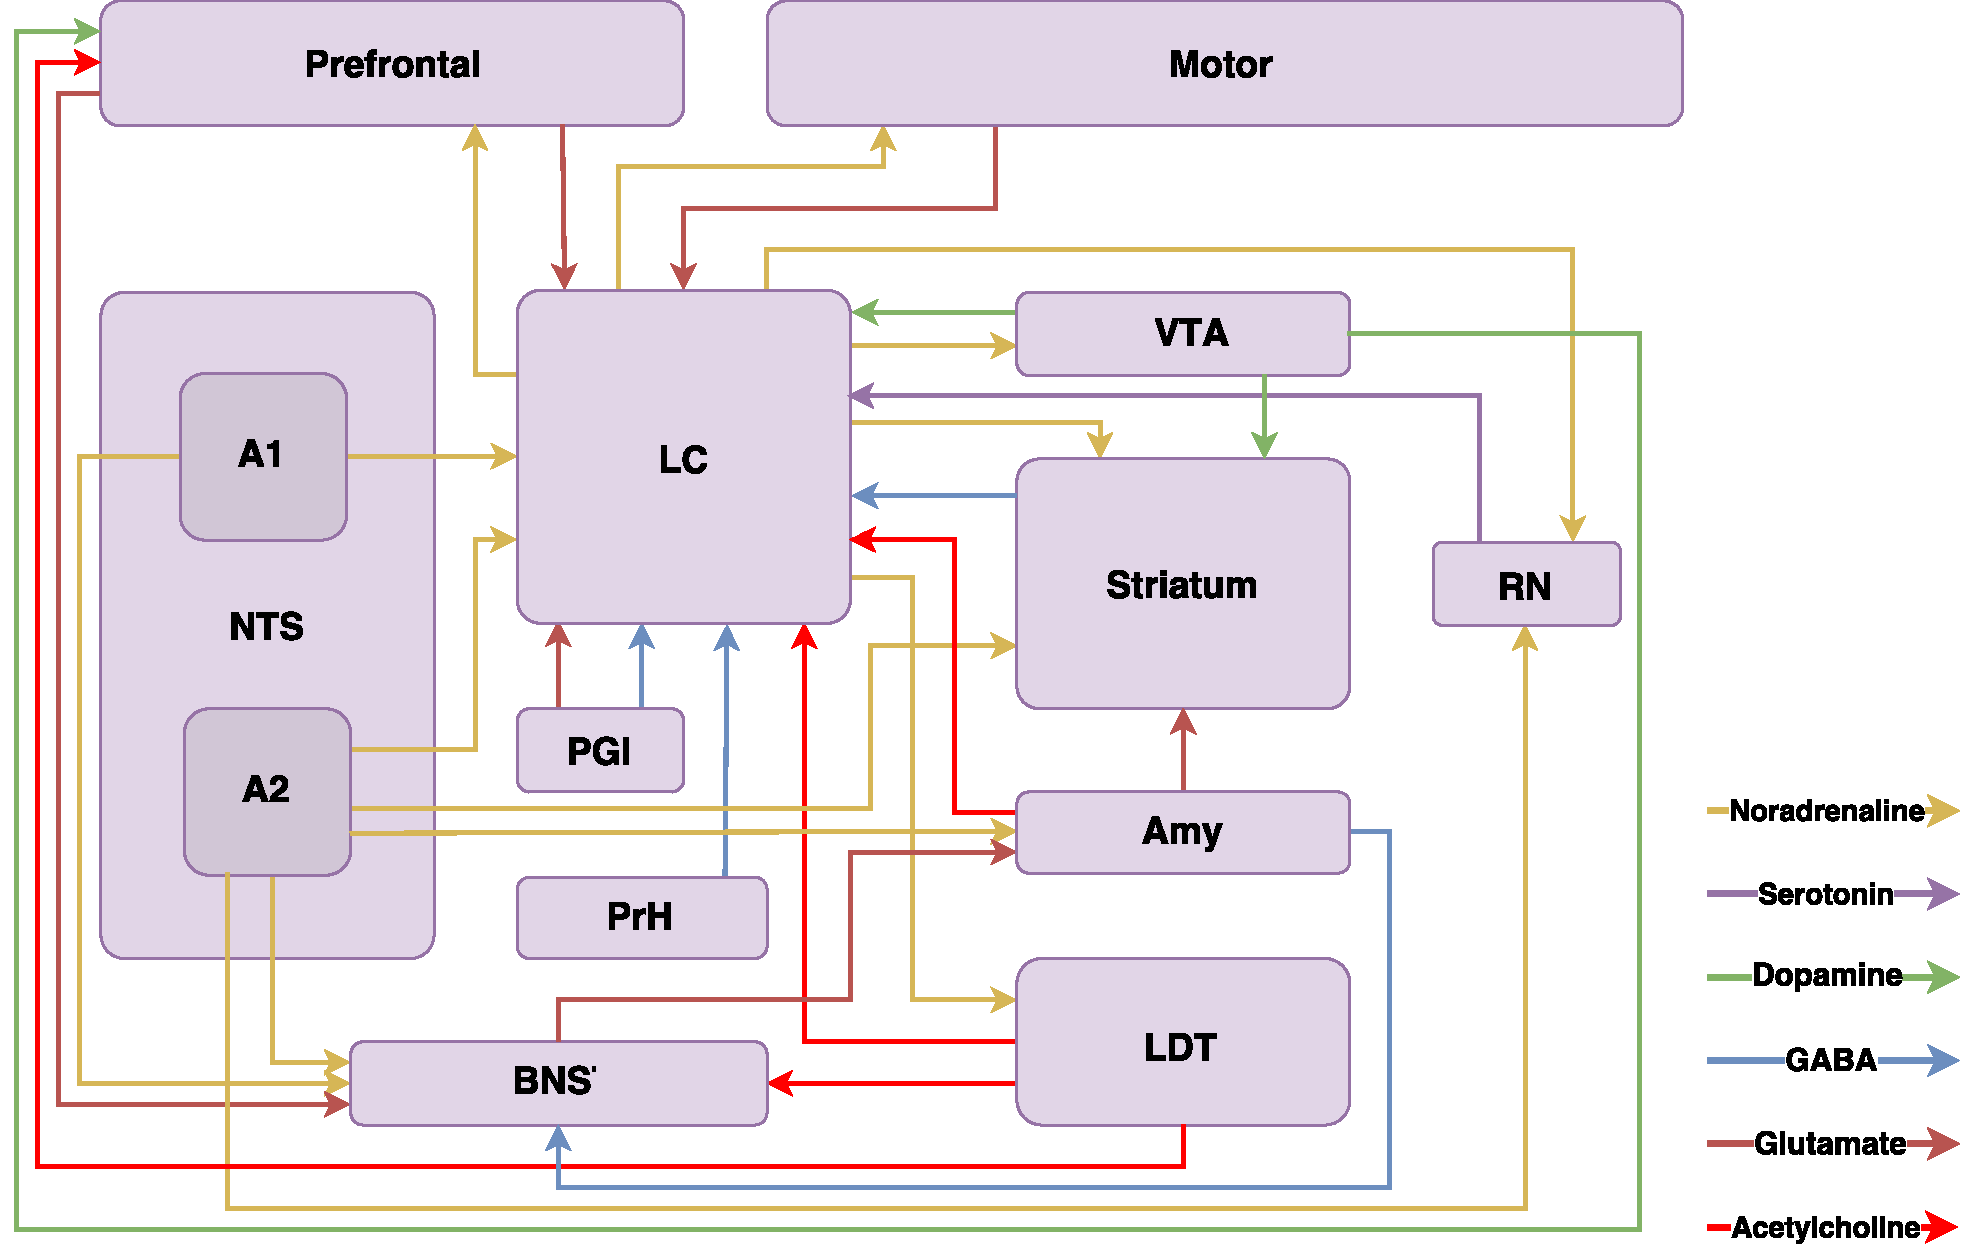
\includegraphics[width=0.8\linewidth]{NA_diagram}
\end{figure}
\end{frame}

%------------------------------------------------
\section{NeuCogAr results}
%------------------------------------------------

\begin{frame}
\frametitle{Dopamine results}
\begin{figure}
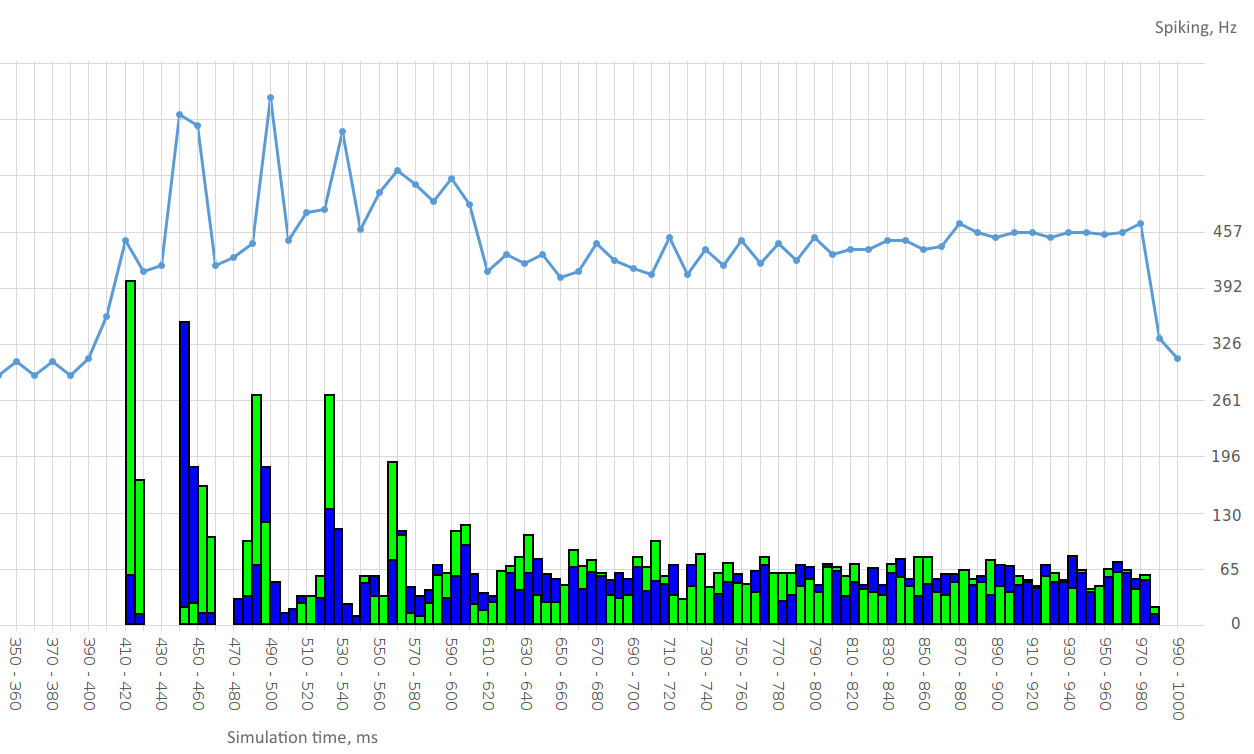
\includegraphics[width=0.8\linewidth]{resultBIG_short}
\end{figure}
\end{frame}

%------------------------------------------------
%------------------------------------------------

\begin{frame}
\frametitle{Serotonin results}
\begin{figure}
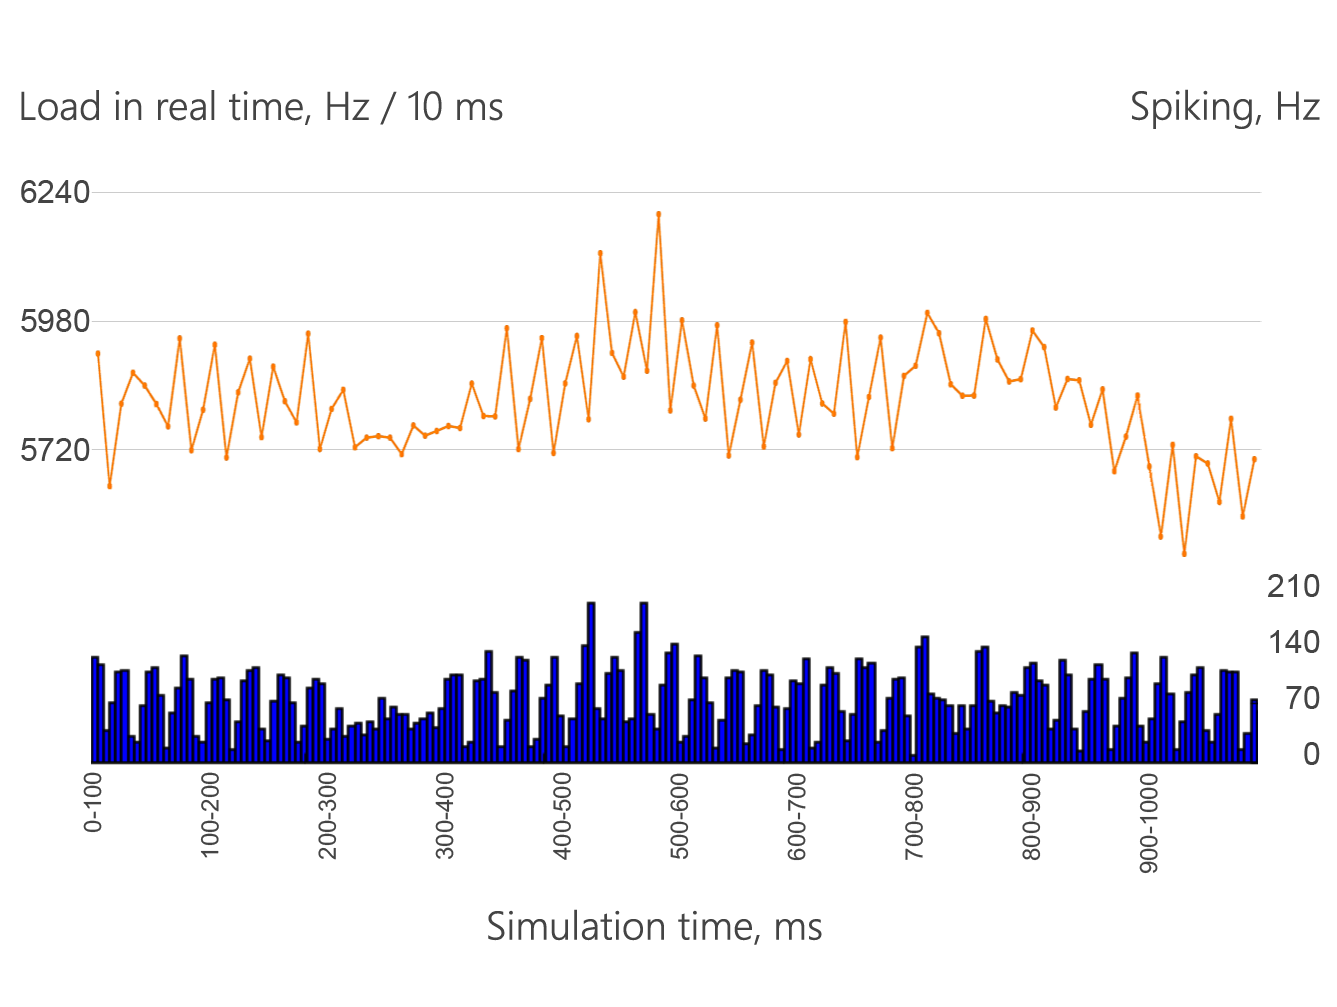
\includegraphics[width=0.8\linewidth]{5ht_results}
\end{figure}
\end{frame}

%------------------------------------------------
%------------------------------------------------

\begin{frame}
\frametitle{Noradrenaline results: prefrontal}
\begin{figure}
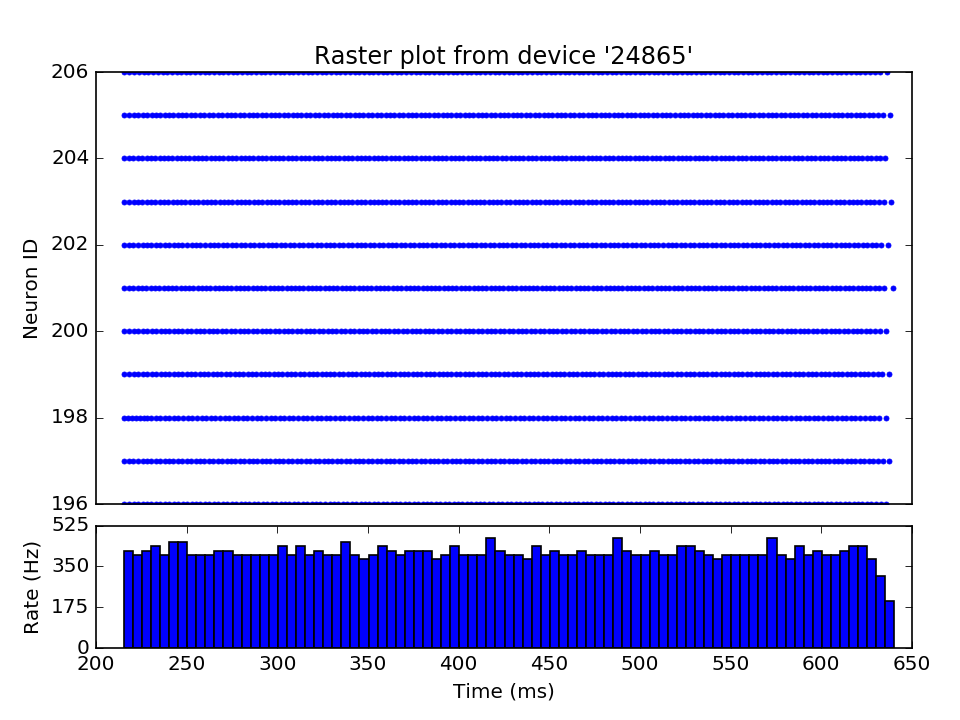
\includegraphics[width=0.7\linewidth]{spikes_prefrontal}
\end{figure}
\end{frame}

%------------------------------------------------
%------------------------------------------------

\begin{frame}
\frametitle{Noradrenaline results: VTA}
\begin{figure}
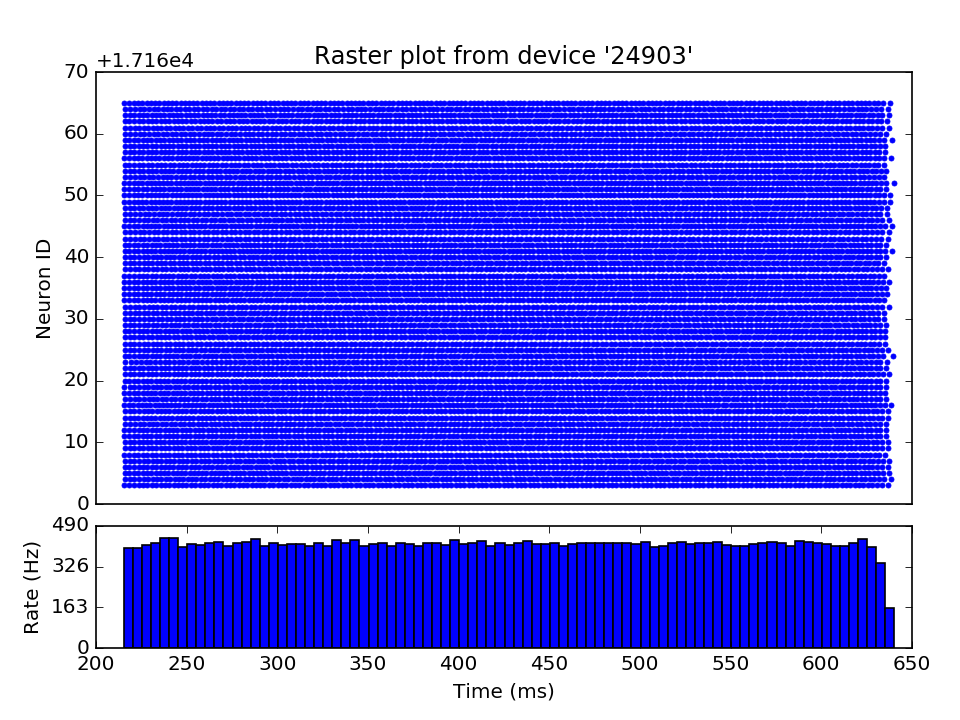
\includegraphics[width=0.7\linewidth]{spikes_vta}
\end{figure}
\end{frame}

%------------------------------------------------
\section{Embodiment}
%------------------------------------------------

\begin{frame}
\frametitle{Robot performance}
\begin{columns}[c] % The "c" option specifies centered vertical alignment while the "t" option is used for top vertical alignment
\column{.45\textwidth} % Left column and width
\begin{itemize}
\item \textbf{AR-601}: Intel Core i7-4700EQ; 8 GB;
\item \textbf{REEM-C}: Intel Core i7 2710QE x 2;
\item \textbf{Nao}: Intel Atom @ 1.6 GHz;
\item \textbf{iCub}: Intel® Core™2 Duo; 2 GB;
\end{itemize}

\column{.6\textwidth} % Right column and width
%------------------------------------------------
\begin{figure}
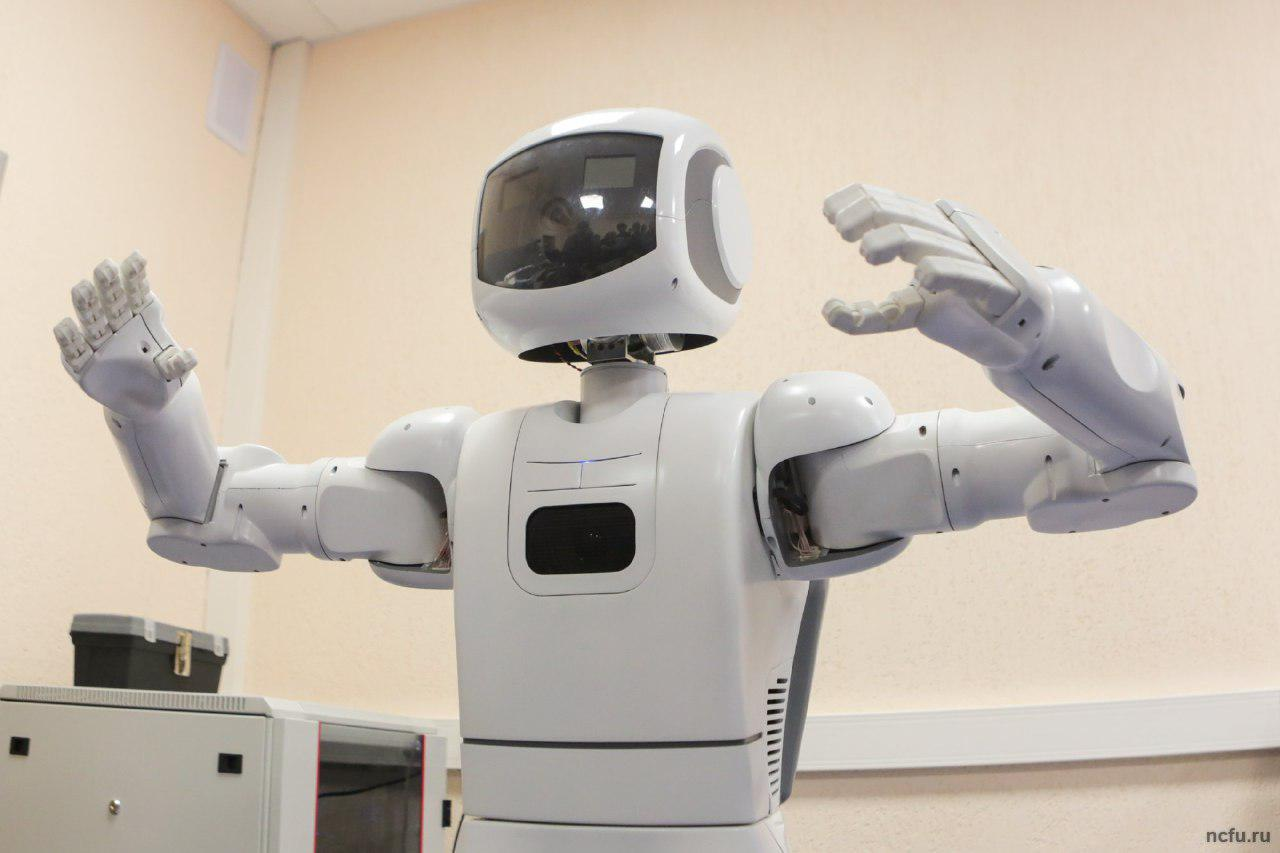
\includegraphics[width=1.0\linewidth]{AR-601}
\end{figure}
%------------------------------------------------
\end{columns}
\end{frame}

%------------------------------------------------

\begin{frame}
\frametitle{Performance that we need}
\begin{columns}[c] % The "c" option specifies centered vertical alignment while the "t" option is used for top vertical alignment
\column{.45\textwidth} % Left column and width
\textbf{RIKEN} 2013: 1\% of human brain - 250 K-supercomputers
(96 computing nodes, 2.0 GHz 8-core SPARC64; 16 GB of memory), slower than human brain in 1000 times.

\textbf{Human brain project}: a whole human brain -- 10 exaflop.

\column{.6\textwidth} % Right column and width
%------------------------------------------------
\begin{figure}
\includegraphics[width=1.0\linewidth]{RIKEN_AICS}
\end{figure}
%------------------------------------------------
\end{columns}
\end{frame}

%------------------------------------------------
\section{Robot dream architecture}
%------------------------------------------------

\begin{frame}
\frametitle{Robot dream architecture}
\begin{figure}
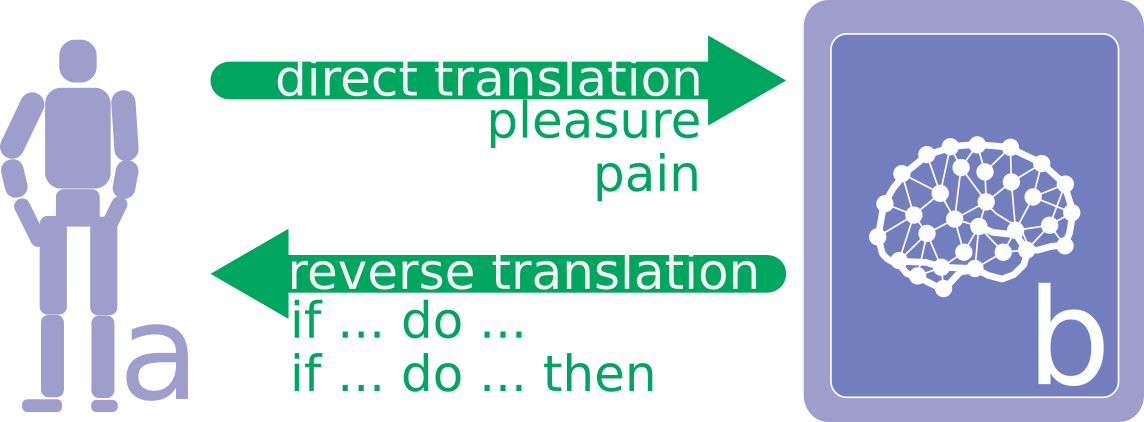
\includegraphics[width=0.8\linewidth]{robot-dream_translations}
\end{figure}
\end{frame}

%------------------------------------------------
%------------------------------------------------

\begin{frame}
\frametitle{Robot dream architecture: lifecycle}
\begin{figure}
\includegraphics[width=0.8\linewidth]{HLD_Activity_life_cycle}
\end{figure}
\end{frame}

%------------------------------------------------
%------------------------------------------------

\begin{frame}
\frametitle{Robot dream architecture: Dremaing brain}
\begin{figure}
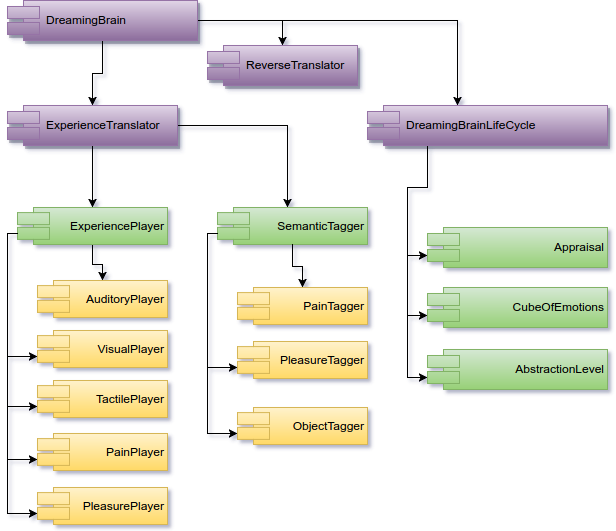
\includegraphics[width=0.6\linewidth]{HLD_Component_MemristiveDreamingBrain.png}
\end{figure}
\end{frame}

%------------------------------------------------
%------------------------------------------------

\begin{frame}
\frametitle{Robot dream architecture: Semantic tagger}
\begin{figure}
\includegraphics[width=0.35\linewidth]{HLD_Activity_SemanticTagger.png}
\end{figure}
\end{frame}

%------------------------------------------------
%------------------------------------------------

\begin{frame}
\frametitle{Pseudo-neuronal activity}
\begin{figure}
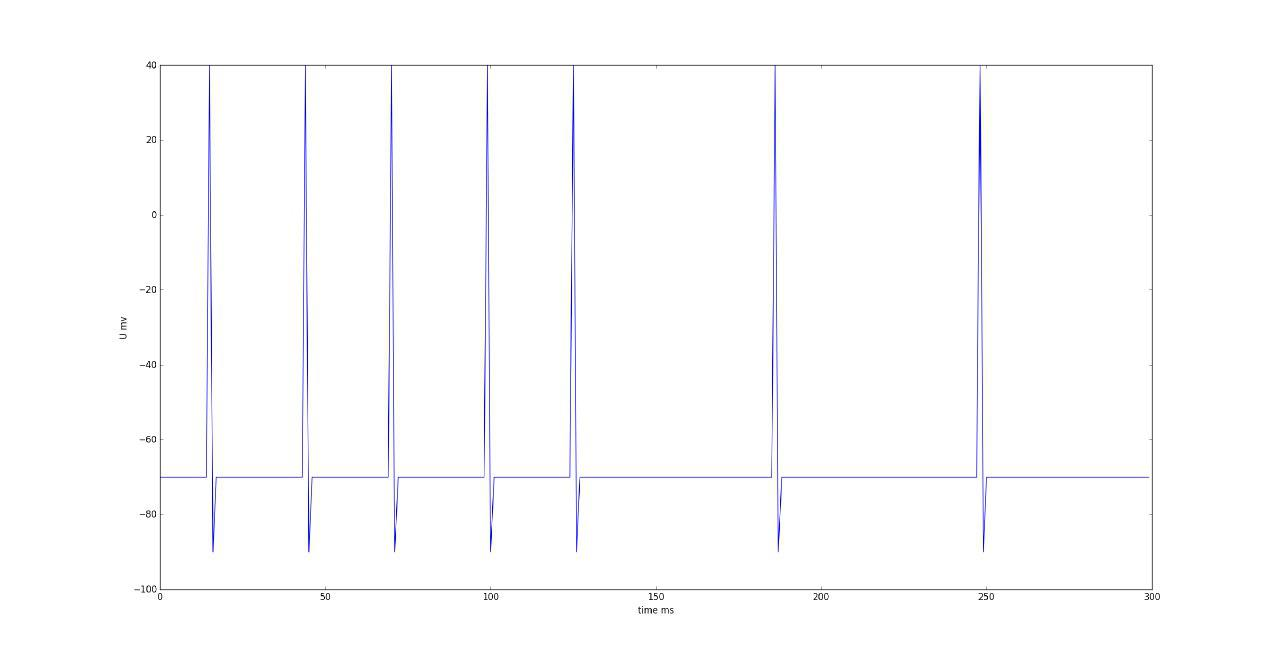
\includegraphics[width=0.8\linewidth]{pseudo-neuronal-activity}
\end{figure}
\end{frame}

%------------------------------------------------
%------------------------------------------------

\begin{frame}
\frametitle{Playback system}
\begin{figure}
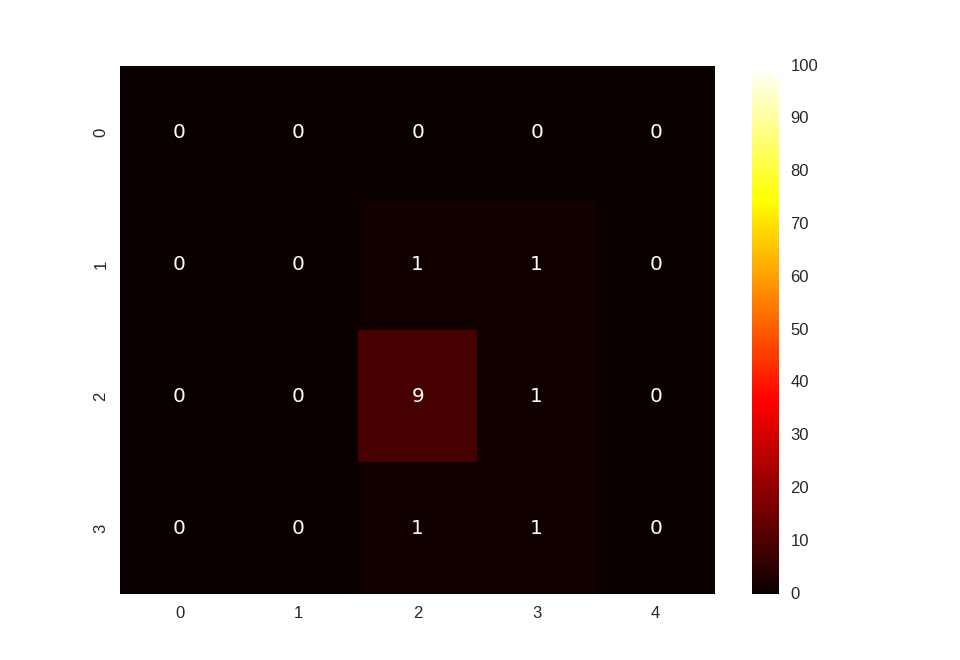
\includegraphics[width=0.33\textwidth]{layer5A_1}
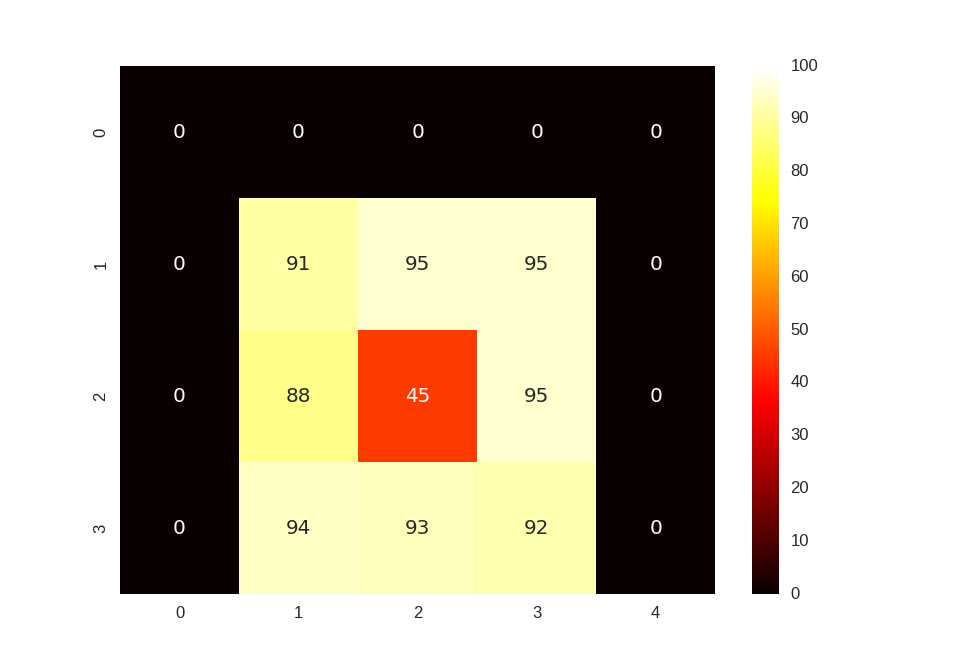
\includegraphics[width=0.33\textwidth]{layer5A_2}
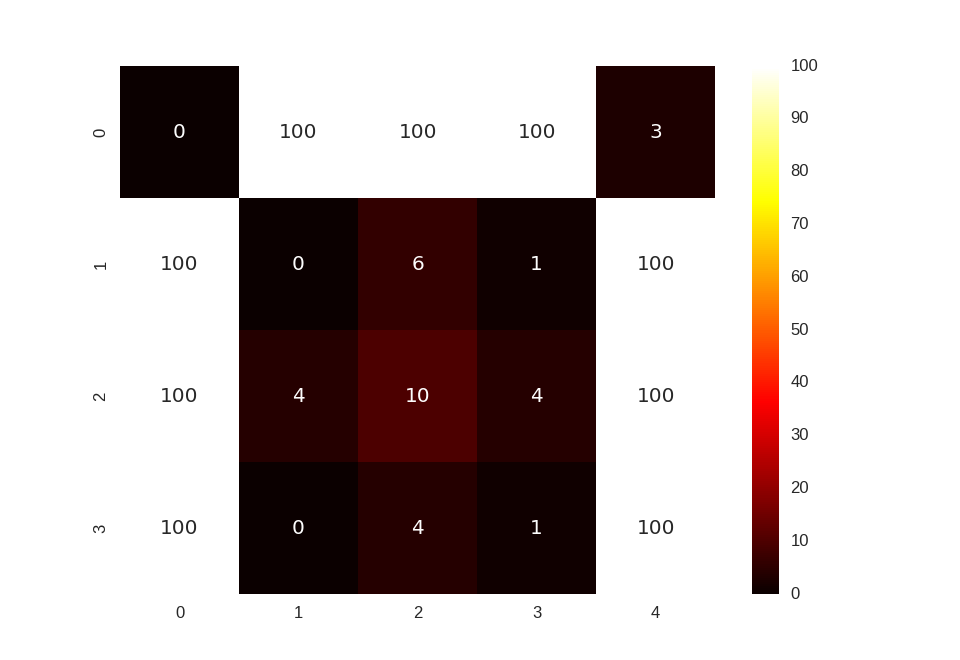
\includegraphics[width=0.33\textwidth]{layer5A_3}
%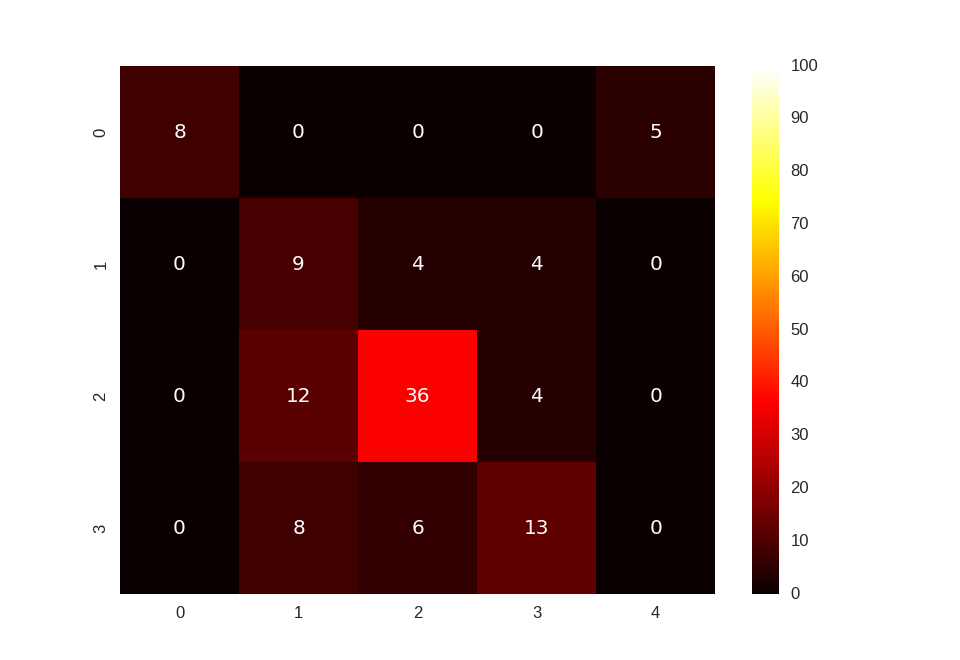
\includegraphics[width=0.25\textwidth]{layer5A_4}
\end{figure}
\end{frame}

%------------------------------------------------
\section{Memristive brain}
%------------------------------------------------

\begin{frame}
\frametitle{Memristive neuron: block diagram}
\begin{figure}
\includegraphics[width=0.8\linewidth]{HL_Emristor}
\end{figure}
\end{frame}

%------------------------------------------------
%------------------------------------------------

\begin{frame}
\frametitle{Memristive neuron: wiring schematic}
\begin{figure}
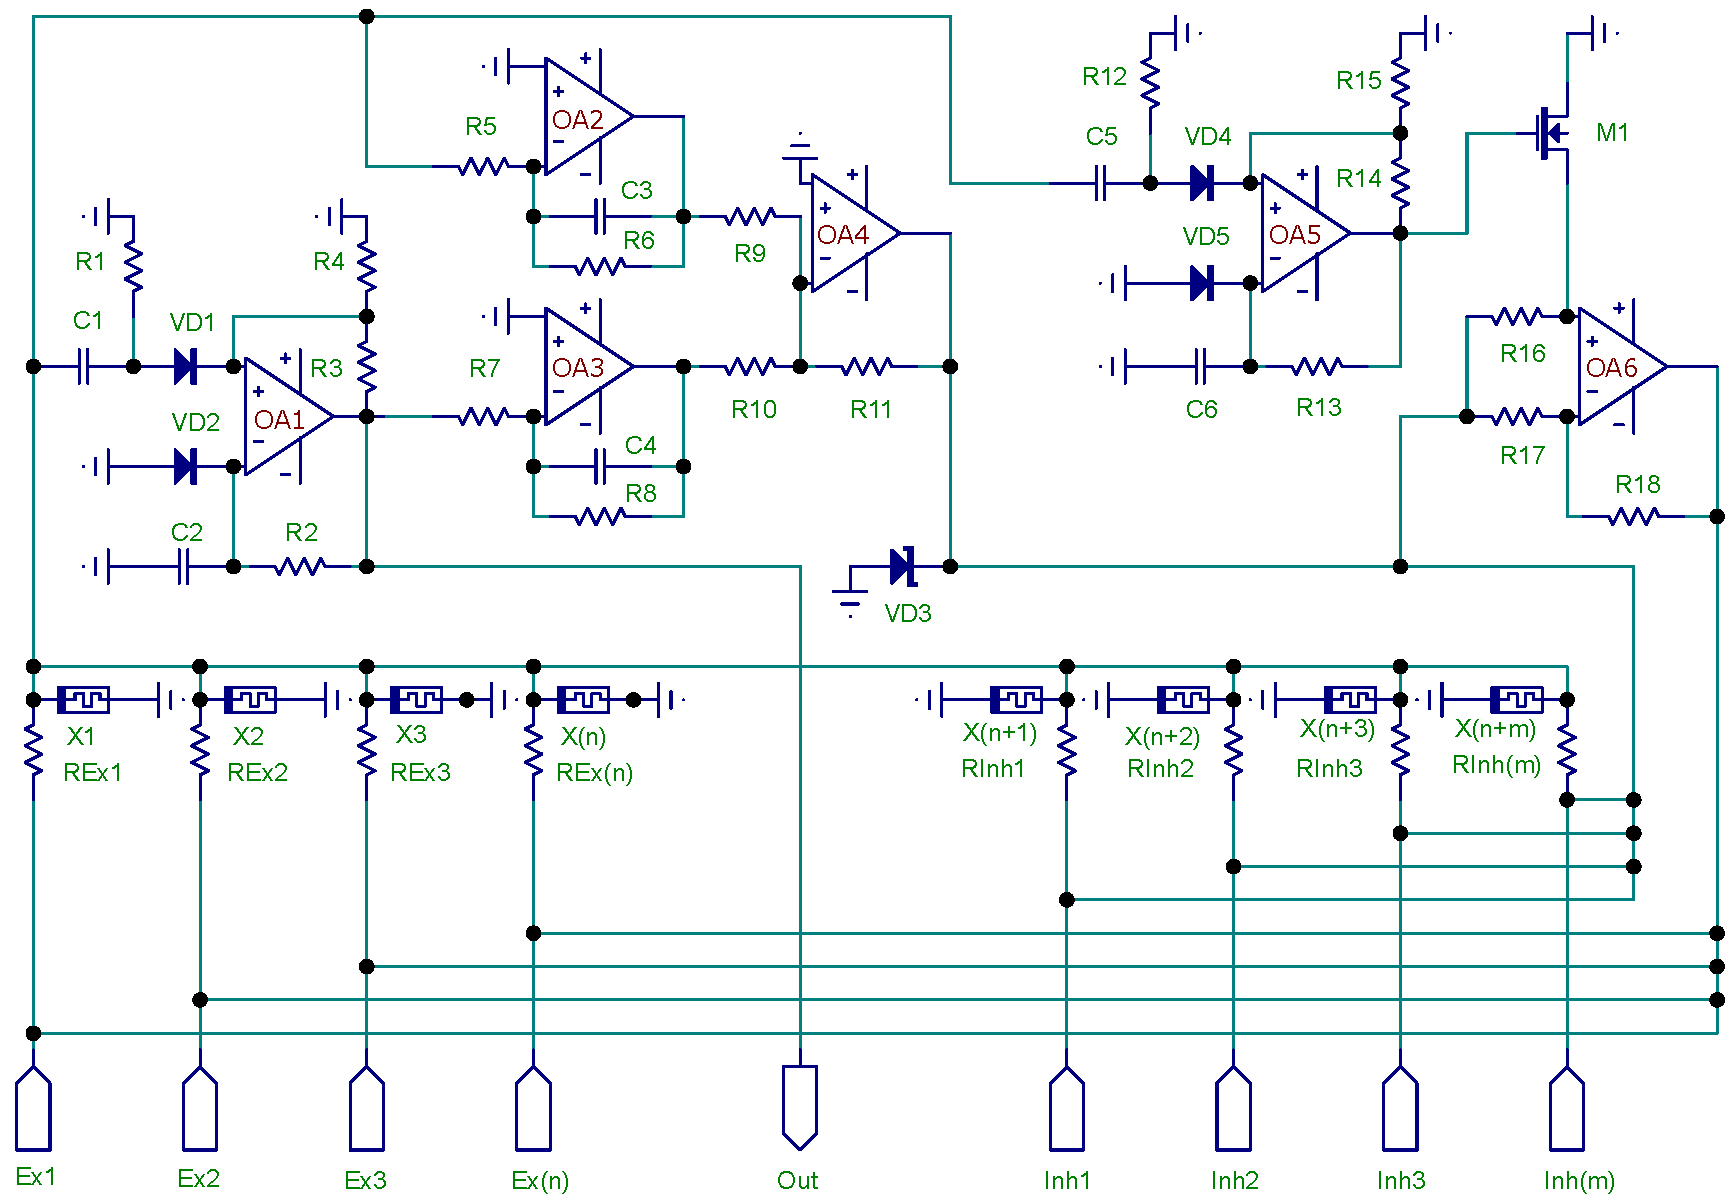
\includegraphics[width=0.7\linewidth]{memristive_neuron_wiring}
\end{figure}
\end{frame}

%------------------------------------------------
%------------------------------------------------

\begin{frame}
\frametitle{Inhibitory ``sombrero'' learning}
\begin{figure}
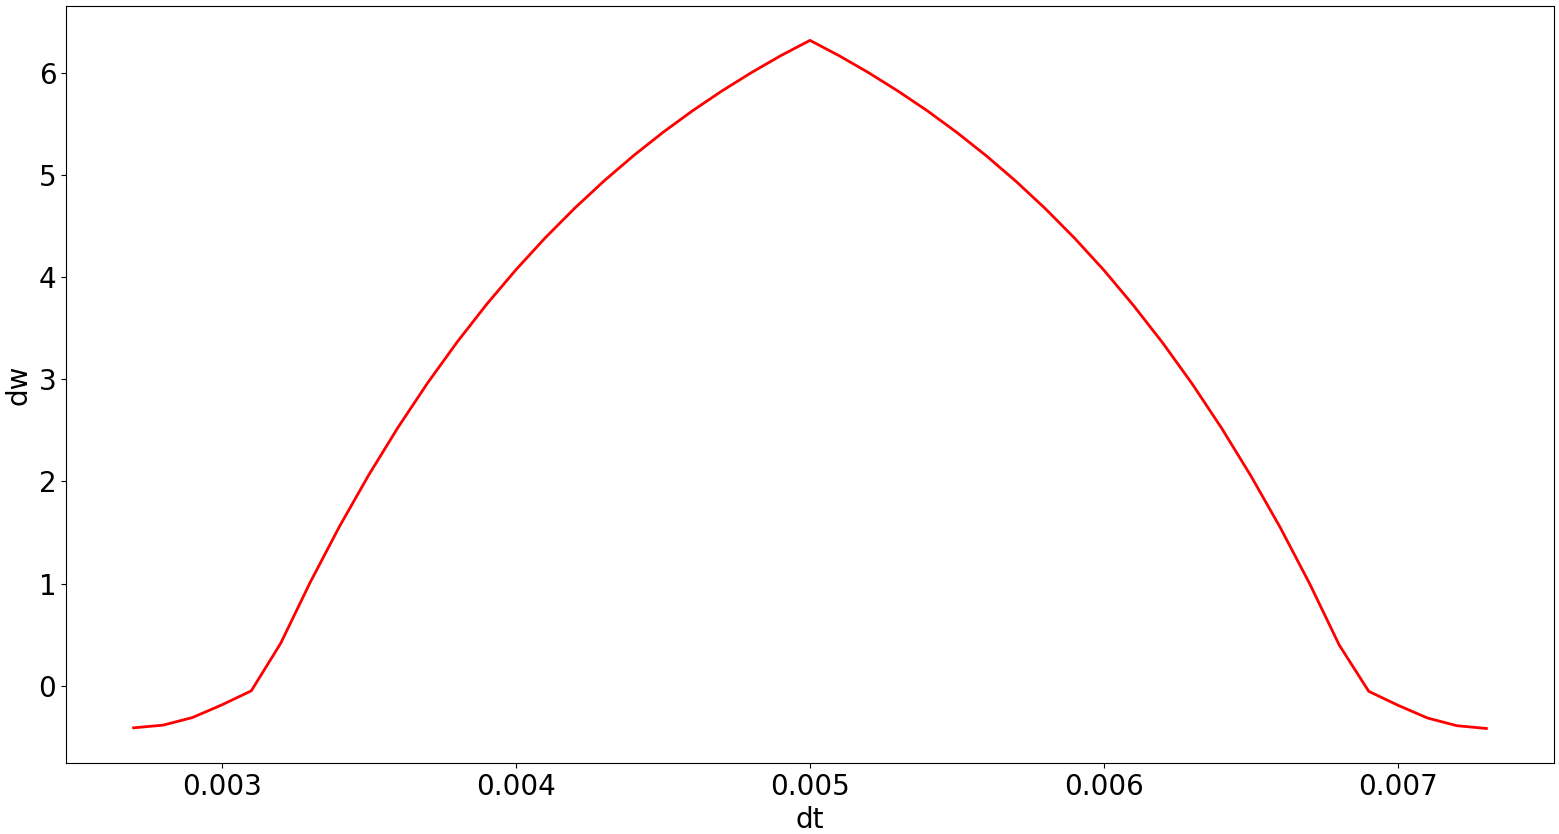
\includegraphics[width=0.9\linewidth]{result_sombrero}
\end{figure}
\end{frame}

%------------------------------------------------
%------------------------------------------------

\begin{frame}
\frametitle{Excitatory (Hebbian) learning}
\begin{figure}
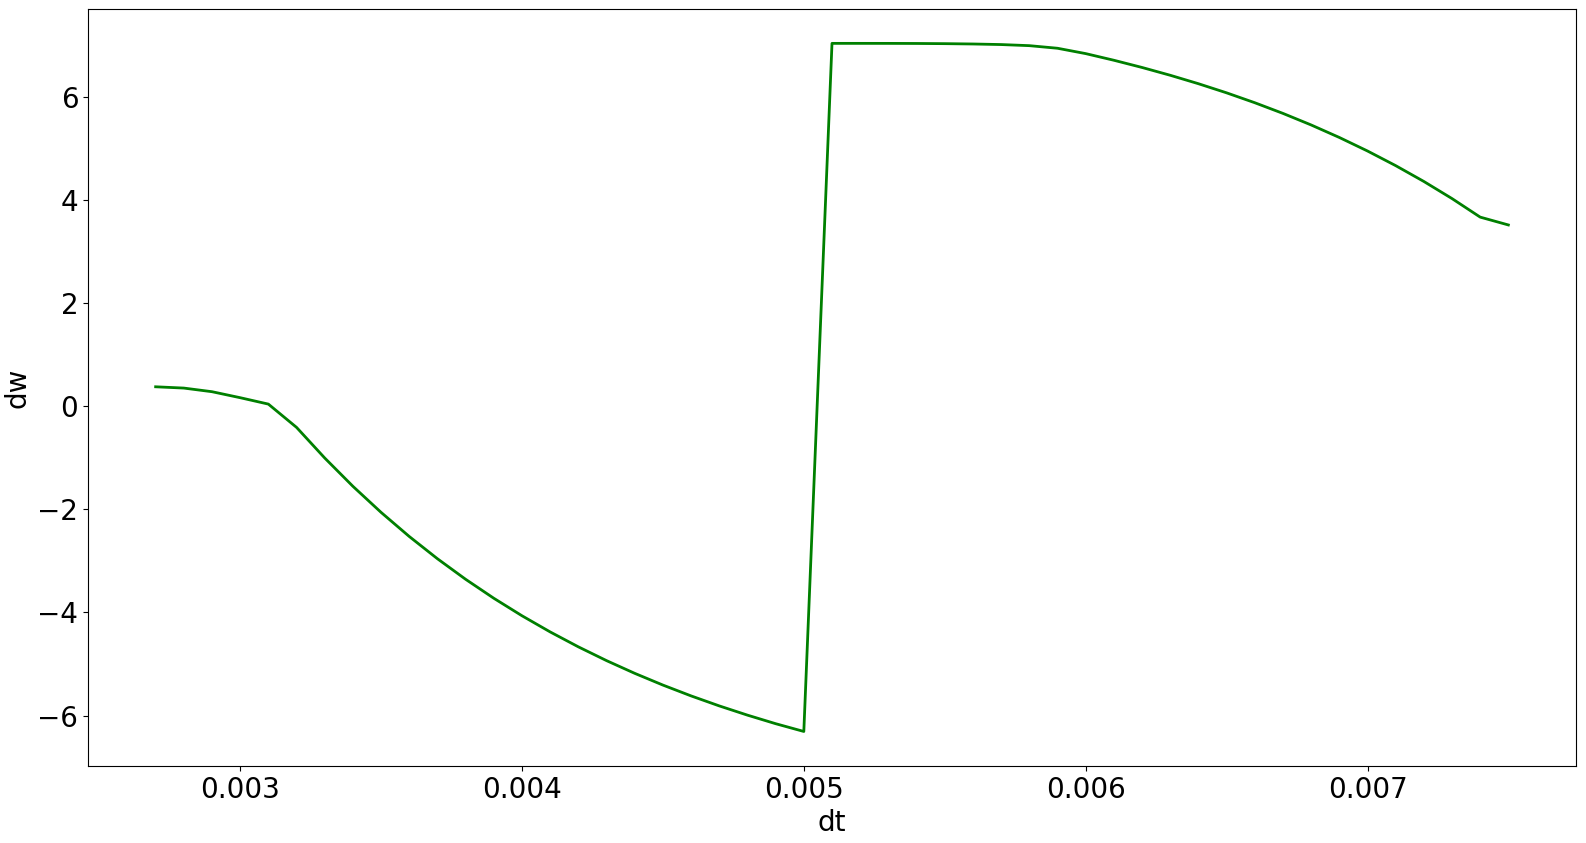
\includegraphics[width=0.9\linewidth]{result_hebb}
\end{figure}
\end{frame}

%------------------------------------------------
\section{Future work}
%------------------------------------------------
\begin{frame}
  \frametitle{Future work}
  
\begin{itemize}
  \item Simple prototype as feasibility study.
  \item \ldots\
  \item Emotional robot with real-time embodiment
  \item Social robot with emotions
  \item Conscious social robot
\end{itemize}

\textbf{Acknowledgment}

Part of the work was performed according to the Russian Government Program of Competitive Growth of Kazan Federal University.


\end{frame}

%------------------------------------------------

%------------------------------------------------

\end{document} 
